%%
%
% ARQUIVO: main.tex
%
% VERSÃO: 1.0
% DATA: Maio de 2016
% AUTOR: Coordenação de Trabalhos Especiais SE/8
% 
%  Arquivo tex principal do documento de Projeto de Fim de Curso (PFC).
%  Este arquivo SÓ PRECISA SER MODIFICADO NA PARTE DE CONTEÚDO:
%
%    a. colocar um \include{•} para cada capítulo do documento de PFC.
%
%%

% -----
% CLASSE DO DOCUMENTO DE PFC
% -----
\documentclass{pfc}

% -----
% PACOTES LATEX USADOS NO DOCUMENTO DE PFC
% -----
\usepackage[brazilian]{babel}
\usepackage[utf8]{inputenc}
\usepackage[T1]{fontenc}

\usepackage{amsmath}
\usepackage{graphicx}
\usepackage{tabularx}
\usepackage{float}
\usepackage{color}
\usepackage{amsfonts,amssymb}
\usepackage[authoryear]{natbib}

\usepackage{enumitem}
\usepackage{rotating}
\usepackage{lipsum}
\usepackage{lastpage}
\usepackage{stringstrings}
\usepackage{pgffor}
\usepackage{pdftexcmds}

% -----
% MARGENS DO DOCUMENTO DE PFC
% -----
\usepackage{geometry}
\geometry{
	a4paper,
	total={210mm,297mm},
	left=25mm,
	right=25mm,
	top=25mm,
	bottom=30mm,
	textwidth=160mm,
	textheight=242mm,
	headheight=0mm,
	headsep=0mm,
}

% -----
% DECLARAÇÕES AUXILIARES PARA REFERÊNCIAS
%
%  Diferencia \citet e \citep de acordo com a NBR 10520:2002
% -----
\DeclareRobustCommand{\NATand}{;}
\DeclareRobustCommand{\NATetal}{et~al.}
\makeatletter
\renewcommand{\NAT@nmfmt}[1]{%
  \ifNAT@swa\expandafter\MakeUppercase
  \else\DeclareRobustCommand{\NATand}{ e}\expandafter\@firstofone\fi{{\NAT@up #1}}%
}
\makeatother

% -----
% AMBIENTE DE FIGURAS DE PFC
%
%  A classe do documento está configurada SOMENTE para figuras no formato EPS.
%  Logo, use PREFERENCIALMENTE este tipo de arquivo.
%
%    a. os arquivos das figuras devem estar no diretório 'img'
% -----
\graphicspath{{./img/}}

% -----
% INÍCIO DO DOCUMENTO DE PFC
% -----
\begin{document}

% -----
% PARTE PRÉ-TEXTUAL DE PFC
%
% Alterar o CONTEÚDO dos arquivos siglas.tex E pre-texto.tex
% -----
%%
%
% ARQUIVO: dados-pfc.tex
%
% VERSÃO: 1.0
% DATA: Maio de 2016
% AUTOR: Coordenação de Trabalhos Especiais SE/8
% 
%  Arquivo tex com os dados acerca do documento de PFC e da apresentação.
%
%   nos campos que definem nomes (autor; orientador; co-orientador; membros da banca)
%   É PRECISO usar os COMANDOS LaTeX para acentuação, conforme abaixo:
%
%         \'a - á || \`a - à || \~a - ã || \^a - â 
%         \'e - é || \^e - ê || \'i - í 
%         \'o - ó || \~o - õ || \^o - ô 
%         \'u - ú || \"u - ü
%
%%

%%% AUTORES DO PFC (Nome completo)
% ---
%  aceita até 03 autores (de autorI até autorIII)
%    a. preencher sucessivamente a partir de autorI
%    b. REMOVER as definições não necessárias
% ---
\autorI{Lucas Menezes Oliveira Sousa}

%%% POSTOS DOS AUTORES DO PFC
% ---
%  aceita os postos de até 03 autores (de postoautorI até postoautorIII)
%    a. preencher sucessivamente a partir de postoautorI (que deve ser o posto de autorI)
%    b. se o autorX É CIVIL, NÃO DEFINIR postoautorX (remover a linha de definição)
%    c. se o autorX É MILITAR, DEFINIR postoautorX com UMA das seguintes ALTERNATIVAS: Alu / 1 Ten / Cap
% ---
\postoautorI{}

%%% TITULO DO PFC
\titulo{Compilando para Brainfuck}


%%% DATA DA APRESENTAÇÃO (formato {dd}{Mmmmm}{aaaa})
\datadefesa{31}{Janeiro}{2018}

%%% ORIENTADOR DO PFC
% ---
%  CAMPO 1: P (para Prof.); PA (para Profa.); ou qualquer coisa (inclusive VAZIO) - o que for escrito aparecerá no documento
%  CAMPO 2: Nome completo
%  CAMPO 3: D (para D.Sc.); P (para Ph.D.); M (para M.Sc.) ou qualquer coisa (inclusive VAZIO) - o que for escrito aparecerá no documento
%  CAMPO 4: Instituição (com "do / da")
% ---
\orientador{P}{Roberto Ierusalimschy}{D}{da PUC-Rio}

%%% CO-ORIENTADOR DO PFC
% ---
%  se não houver co-orientador, REMOVA ESTA LINHA
%  preenchimento idêntico a \orientador{}{}{}{}
% ---

%%% NÚMERO DA ENTRADA DA BIBLIOTECA (pegar na Biblioteca do IME)
\biblioref{004.69}{S586e}

%%% PALAVRAS-CHAVES DO PFC
% ---
%  devem ser separadas por vírgula e É OBRIGATÓRIO ter pelo menos uma
% ---
\palavraschaves{Palavra 01, Palavra 02, Palavra 03}

%%% OUTROS MEMBROS DA BANCA DO PFC
% ---
%  aceita até mais 05 membros (de membrobancaI até membrobancaV)
%    a. preencher sucessivamente a partir de membrobancaI
%    b. REMOVER as definições não necessárias
%
%  cada membro tem preenchimento idêntico a \orientador{}{}{}{}
% ---
\membrobancaI{}{Nome do Membro da Banca 1}{}{da PUC-Rio}
\membrobancaII{P}{Nome do Membro da Banca 2}{M}{do Massachussets Institute of Technology}
%\membrobancaIII{}{Nome do Membro da Banca 3}{}{da COPPE/UFRJ}
%\membrobancaIV{}{Nome do Membro da Banca 4}{}{da UNIRIO}
%\membrobancaV{}{Nome do Membro da Banca 5}{}{da UERJ}

%%
%
% ARQUIVO: pre-texto.tex
%
% VERSÃO: 1.0
% DATA: Maio de 2016
% AUTOR: Coordenação de Trabalhos Especiais SE/8
% 
%  Arquivo tex para a criação da parte pré-textual do documento de Projeto de Fim de Curso.
%
%%


% -----
% PÁGINA DE CAPA DO DOCUMENTO DE PFC
% -----
\makecapa

% -----
% PÁGINA DE TÍTULO DO PFC
% -----
\prepareadvisors
\maketitle

% -----
% PÁGINA DE CRÉDITOS DO DOCUMENTO DE PFC
% -----

% -----
% PÁGINA DE FOLHA DE ASSINATURAS
% -----
\preparemembers

% -----
% PÁGINA DE DEDICATÓRIA (OPCIONAL, ie. pode remover toda a página)
% -----
%%% DEDICATÓRIA - PREENCHER...

% -----
% PÁGINA DE AGRADECIMENTOS (OPCIONAL, ie. pode remover toda a página)
% -----
%%% AGRADECIMENTOS - PREENCHER...
\agradecimentos{%
Agradeço ao Professor Roberto, por ter me mostrado o ramo de estudos sobre as linguagens de programação.  \\
\indent
Agradeço ao Professor Ivan, por ter me ensinado a codificar, que tanto tentei aprender sozinho sem sucesso.\\
\indent
Agradeço especialmente aos desenvolvedores do Valgrind, que possibilitaram a escrita deste software. \\
\indent
Agradeço especialmente aos contribuidores da esolangs.org, que escreveram os códigos da página \textit{Brainfuck Algorithms} sem os quais esse projeto seria impossível.\\
\\
\indent
Agradeço aos meus professores da PUC por terem fornecido o ambiente no qual eu pude desenvolver tais conhecimentos. 
}%
\makethanks

% -----
% PÁGINA DE EPÍGRAFE (OPCIONAL, ie. pode remover toda a página)
% -----
%%% EPÍGRAFE - PREENCHER...
\epigrafe{%
Os poetas não enlouquecem, mas os jogadores de xadrez, sim.
}%
\autorepigrafe{%    %% Se não tem autor, coloque "Anônimo"
Alan J. Perlis
}%
\epigrafe{%
I think that it's extraordinarily important that we in computer science keep fun in computing. When it started out, it was an awful lot of fun..
}%
\autorepigrafe{%    %% Se não tem autor, coloque "Anônimo"
Alan J. Perlis
}%
\makeepigraph

% -----
% PÁGINA DE SUMÁRIO
% -----
\tableofcontents

% -----
% PÁGINAS DE LISTAS DE FIGURAS E DE TABELAS
% se a Dissertação não possui figuras e/ou tabelas, REMOVA O COMANDO CORRESPONDENTE
% -----


% -----
% PÁGINA DE LISTA DE SIGLAS
% se a Dissertação não possui siglas, REMOVA TODA A PÁGINA
% -----
%%% SIGLAS - PREENCHER...


% -----
% PÁGINA DE LISTA DE ABREVIATURAS
% se a Dissertação não possui abreviaturas ou símbolos, REMOVA TODA A PÁGINA
% -----
%%% ABREVIATURAS - PREENCHER...


% -----
% PÁGINA DE RESUMO
% -----
%%% RESUMO - PREENCHER...
\resumo{%
Menezes Lucas. Ierusalimschy Roberto, Compilando pra Brainfuck – A Linguagem Headache - 44 páginas - Pontifícia Universidade Católica do Rio de Janeiro.
Este documento descreve a linguagem de programação Headache e o seu compilador, hac (Headache Compiler).  Headache é uma linguagem de programação estruturada (bastante parecida com C) que é compilada para brainfuck de 8 bits. Neste documento é discutido como foi implementado, quais foram as técnicas, o modelo de memória e as estratégias utilizadas para fazer o sistema funcionar.\\
\\
Palavras-chaves: Brainfuck, Headache, Compilador, Linguagem de Programação.
}%
\makeresumo

% -----
% PÁGINA DE ABSTRACT
% -----
%%% ABSTRACT - PREENCHER...
\abstract{%
Menezes Lucas. Ierusalimschy Roberto, Compiling to Brainfuck – The Headache Programming Language -  44 pages - Pontifícia Universidade Católica do Rio de Janeiro
This document describes the Headache Programming Language and its compiler, hac (Headache Compiler). Headache is a structured programming Language (which is very C-like) that is compiled to 8 bit brainfuck. In this document we discuss how it was implemented, the structures that were used, its memory model and the strategy used to bring everything working together.\\
\\
Keywords: Brainfuck, Headache, Compiler, Programming Language.
}%
\makeabstract


\parindent 0.75cm

% -----
% PARTE DE CONTEÚDO DE PFC
%
%  Escrever cada capitulo do documento de PFC em um arquivo .tex separado.
%  Adicionar os arquivos .tex ao documento com comando \include{•}
% -----
%%
%
% ARQUIVO: cap-01.tex
%
% VERSÃO: 1.0
% DATA: Maio de 2016
% AUTOR: Coordenação de Trabalhos Especiais SE/8
% 
%  Arquivo tex de exemplo de capítulo do documento de Projeto de Fim de Curso.
%
% ---
% DETALHES
%  a. todo capítulo deve começar com \chapter{•}
%  b. usar comando \noindent logo após \chapter{•}
%  c. citações para referências podem ser
%       i. \citet{•} para citações diretas (p. ex. 'Segundo Autor (2015)...'
%       ii. \citep{•} para citações indiretas (p. ex. '... (AUTOR, 2015)...'
%  d. notas de rodapé devem usar dois comandos
%       i. \footnotemark para indicar a marca da nota no texto
%       ii. \footnotetext{•}, na sequência, para indicar o texto da nota de rodapé
%  e. figuras devem seguir o exemplo
%       i. devem ficar no diretório /img e devem ser no formato EPS
%  f. tabelas devem seguir o exemplo
%  g. figuras e tabelas podem ser colocadas em orientação landscape
%       i. figuras: usar \begin{sidewaysfigure} ... \end{sidewaysfigure}
%                   em vez de \begin{figure} ... \end{figure}
%       ii. tabelas: usar \begin{sidewaystable} ... \end{sidewaystable}
%                    em vez de \begin{table} ... \end{table}
%  h. toda figura e tabela deve ser referenciada ao longo do texto com \ref{•}
% ---
%%

\chapter{Introdução}
\noindent

É muito difícil elaborar programas em \textit{brainfuck}. Porém, é fácil programar em linguagens estruturadas. Portanto se propõe a criação de uma linguagem estruturada (\textbf{\textit{Headache}}) cujo compilador gere código \textit{brainfuck}.				

A linguagem \textit{brainfuck} é uma das mais simples representações de uma máquina de Turing. Assim, \textit{Headache} poderia ser útil como exemplo de completude-Turing (Turing-completeness), uma vez que mostra que um código genérico é passível de ser transformado em 8 instruções simples. No entanto, esse objetivo é secundário.

O objetivo primário deste trabalho é o estudo de elaboração de linguagens de programação e de técnicas de compilação e otimização. \textit{Brainfuck} é utilizada aqui como contexto de desafio técnico. Tal trabalho permite o exercício de diversos conteúdos aprendidos no curso, desde estruturas de dados, até prática de teste de software. 	

\section{Projetos similares}
Há projetos similares a \textit{Headache} que são dignos de nota: \textit{Brain} é uma linguagem com a sintaxe similar à linguagem \textit{Rust} que compila para \textit{Brainfuck}. \textit{Headache} se diferencia de \textit{Brain} por ter a sintaxe similar a C e monga além de focar majoritariamente em ser uma distribuição tão leve e tão fácil de instalar quanto possível.

\section{Sobre o ambiente computacional}
O sistema está sendo desenvolvido em ambiente unix, (mais especificamente em um computador \textit{Mac OS Sierra}). Para edição de código é utilizado o \textit{Sublime Text 3}. A compilação é regida por um arquivo \textit{Makefile}. Não há IDE. Os testes são regidos por scripts \textit{shell}. O projeto é versionado utilizando \texit{git} e possui um repositório público no \textit{github}. O projeto foi desenvolvido em \textit{C99}. O analisador léxico e o analisador sintático foram desenvolvidos utilizando o \textit{flex} e o \textit{bison} respectivamente. Há um arquivo de descrição de \textit{tokens} (\textit{rules.lex}) e um arquivo de regras sintáticas e criação da AST (\textit{grammar.y}) ambos geram arquivos .c que são compilados conjuntamente aos outros arquivos fonte.

Assim, o projeto depende apenas de C99, \textit{Flex, Bison} e \textit{Unix Shell}.

É oportuno destacar aqui que os objetivos ao escolher essas tecnologias são os seguintes: \textit{Flex} e \textit{Bison} são escolhidos aqui porque são ferramentas bem conhecidas e bem documentadas, com as quais trabalhei anteriormente, que resolvem o problema dos analisadores léxico e sintático de uma forma muito satisfatória.

C99 foi escolhido para integrar diretamente os outputs do \textit{Bison} e do \textit{Flex} e por ser uma versão relativamente recente da mesma linguagem. Além disso, compiladores de C costumam vir instalados (ou ser de fácil instalação) em sistemas \textit{unix}. C também é escolhida por sua alta velocidade de execução nas suas instalações padrão.

\textit{Unix Shell} foi escolhida também por já estar presente nos sistemas unix e porque fornece uma maneira fácil de redigir \textit{scripts} aproveitando programas úteis como \textit{rm, mv, cmp} e \textit{diff}.

As tecnologias utilizadas foram decididas por facilidade que algum usuário de um sistema \textit{unix} teria ao tentar clonar o projeto do \textit{github} e tentar executá-lo. \textit{\textbf{Headache}} foi planejada para ser perfeitamente utilizável por um usuário padrão do \textit{github.com} a partir de comandos simples como:

\begin{verbatim}
    git clone https://github.com/LucasMW/Headache
    cd Headache
    make
\end{verbatim}

Caso o usuário não tivesse o \textit{flex} ou o \textit{bison} instalados, os pode instalar com simples comandos como 
\begin{verbatim} apt-get install flex bison \end{verbatim} 
ou 
\begin{verbatim} brew install flex bison \end{verbatim} e rodar novamente os comandos acima.

Nota: Embora \textit{Headache} possa ser compilada para \textit{Windows} e exista um \textit{branch} no \textit{github} dedicado a isso, a \textit{build Windows} não tem suporte oficial.

\section{Adequação do trabalho como Projeto Final}
Este trabalho permitiu o treino de habilidades que são muito úteis no desenvolvimento de \textit{software}. Dentre elas, permitiu o aproveitamento e adaptação de código legado, permitiu o treino de manutenção de repositório \textit{github} (\textit{Headache} tem o \textit{branch master}, além de um \textit{branch} específico para \textit{mac, linux} e \textit{windows}, para gerar os \textit{releases} específicos) assim como cuidar da \textit{wiki} do projeto. Além disso, \textit{Headache} é um desafio técnico considerável, ordens de grandeza mais desafiador do que foi compilar \textit{monga} para \textit{llvm}. 

%%
%
% ARQUIVO: cap-02.tex
%
% VERSÃO: 1.0
% DATA: Maio de 2017
% AUTOR: Carla Cosenza, Matheus Mello, Rebeca Reis
% 
%  Arquivo tex de exemplo de capítulo do documento de Projeto de Fim de Curso.
%
% ---
% DETALHES
%  a. todo capítulo deve começar com \chapter{•}
%  b. usar comando \noindent logo após \chapter{•}
%  c. citações para referências podem ser
%       i. \citet{•} para citações diretas (p. ex. 'Segundo Autor (2015)...'
%       ii. \citep{•} para citações indiretas (p. ex. '... (AUTOR, 2015)...'
%  d. notas de rodapé devem usar dois comandos
%       i. \footnotemark para indicar a marca da nota no texto
%       ii. \footnotetext{•}, na sequência, para indicar o texto da nota de rodapé
%  e. figuras devem seguir o exemplo
%       i. devem ficar no diretório /img e devem ser no formato EPS
%  f. tabelas devem seguir o exemplo
%  g. figuras e tabelas podem ser colocadas em orientação landscape
%       i. figuras: usar \begin{sidewaysfigure} ... \end{sidewaysfigure}
%                   em vez de \begin{figure} ... \end{figure}
%       ii. tabelas: usar \begin{sidewaystable} ... \end{sidewaystable}
%                    em vez de \begin{table} ... \end{table}
%  h. toda figura e tabela deve ser referenciada ao longo do texto com \ref{•}
% ---
%%

\chapter{Situação Atual}
\noindent
Escrever programas em \textit{Brainfuck} é muito difícil. Isso faz com que a biblioteca de exemplos em \textit{Brainfuck} seja muito curta.

Escrever, no entanto, programas de exemplo em linguagens estruturadas é fácil. Já existem algumas soluções que compilam de uma linguagem estruturada para \textit{Brainfuck}, porém são desconhecidas, a maioria dela são apenas soluções pessoais.

\section{Descrição e avaliação de tecnologias e sistemas existentes}
Em 2017, durante o desenvolvimento de Headache, surgiu uma solução similar nomeada \textit{Brain} feita em \textit{Rust}. Ela utiliza a sintaxe inspirada em \textit{Rust} e compila para \textit{Brainfuck}. Headache se diferencia da brain por usar uma sintaxe inspirada em C  (e em monga, por extensão). Além disso, o compilador hac foca em ser uma implementação leve (os binários pesam em torno de 100KB ) e rápida de um compilador, inclusive no tempo de compilação (3 segundos). 

Já a Brain, demora 474.3 segundos para compilar no release,  possui 1,6 MB e mais 12 MB de dependência. 
Existem outras soluções mais antigas como a ebf feitas nos anos 2000, porém estão perdidas em pastas compactadas em páginas antigas da internet. Muitas vezes não tem documentação, ou simplesmente não tem nenhuma usabilidade.

Headache propõe contrapor esse ponto. A usabilidade hac é baseada diretamente na utilização do gcc e do clang. Algumas features como modo interativo foram adicionadas pensando no comportamento das distribuições linguagens interpretadas,.

A usabilidade do repositório é baseada diretamente em padrões de simplicidade do github e de projetos unix. O repositório foi feito justamente para ser clonado, compilado e estar usável em menos de um minuto.

%%
%
% ARQUIVO: cap-02.tex
%
% VERSÃO: 1.0
% DATA: Maio de 2017
% AUTOR: Carla Cosenza, Matheus Mello, Rebeca Reis
% 
%  Arquivo tex de exemplo de capítulo do documento de Projeto de Fim de Curso.
%
% ---
% DETALHES
%  a. todo capítulo deve começar com \chapter{•}
%  b. usar comando \noindent logo após \chapter{•}
%  c. citações para referências podem ser
%       i. \citet{•} para citações diretas (p. ex. 'Segundo Autor (2015)...'
%       ii. \citep{•} para citações indiretas (p. ex. '... (AUTOR, 2015)...'
%  d. notas de rodapé devem usar dois comandos
%       i. \footnotemark para indicar a marca da nota no texto
%       ii. \footnotetext{•}, na sequência, para indicar o texto da nota de rodapé
%  e. figuras devem seguir o exemplo
%       i. devem ficar no diretório /img e devem ser no formato EPS
%  f. tabelas devem seguir o exemplo
%  g. figuras e tabelas podem ser colocadas em orientação landscape
%       i. figuras: usar \begin{sidewaysfigure} ... \end{sidewaysfigure}
%                   em vez de \begin{figure} ... \end{figure}
%       ii. tabelas: usar \begin{sidewaystable} ... \end{sidewaystable}
%                    em vez de \begin{table} ... \end{table}
%  h. toda figura e tabela deve ser referenciada ao longo do texto com \ref{•}
% ---
%%

\chapter{Objetivos}
\noindent
O objetivo é ter a linguagem Headache implementada no compilador hac.
É objetivo deste trabalho que o código gerado pelo hac seja executável em qualquer interpretador brainfuck de 8 bits decente. O interpretador é considerado decente, neste trabalho, se passa pelos testes elaborados por Daniel Cristofani (veja a referência \cite{BrainfuckFluff}). Estes testes estão na source tree de Headache numa suíte de testes própria.	

Objetiva-se ter a linguagem Headache implementada gradualmente. Ao final do prazo de entrega do Projeto Final 2 espera-se que estejam corretamente implementados na linguagem os seguintes recursos funcionando plenamente:

\begin{itemize}
    \item Definição de variáveis de tipo inteiro (byte, short e int)
    \item Expressões aritméticas de tipo inteiro (byte) 
    \item Expressões aritméticas de inteiros de mais de 8 bits (short e int)
    \item Atribuição de expressões a variáveis
    \item Incrementos e Decrementos (++ e --)
    \item Print de valores dinâmicos (constantes e variáveis)
    \item Chamada de funções com e sem parâmetros
    \item Funções com retorno
    \item Condições e operadores lógicos
    \item Comandos If/Else
    \item Comandos While e For
    \item Constantes do tipo String
    \item Print de Strings
    \item Leitura de números do console para variáveis
    \item Cast automático de tipos inteiros
\end{itemize}

Ver também Anexo 1 para uma descrição mais completa das features da linguagem. Há, também, no documento um trecho sobre as features não implementadas.

Além disso, Headache se destina a ser a implementação mais leve de uma linguagem que compila para Brainfuck. Objetiva também ter reconhecimento no github em buscas como 'Brainfuck' e 'esoteric-programming language' e que os entusiastas de Brainfuck e linguagens esotéricas tenham uma distribuição extremamente fácil de instalar. 

Em relação ao estado da arte, Headache é, até o dia da conclusão escrita deste relatório, a única linguagem de programação que apresenta uma solução para compilar tipos inteiros de 16 ou mais bits em Brainfuck de 8 bits em seu código fonte.

Também se almeja que Headache atinja bastante reconhecimento no github e seja referenciada na esolangs.org com menções honrosas.
%%
%
% ARQUIVO: cap-02.tex
%
% VERSÃO: 1.0
% DATA: Maio de 2017
% AUTOR: Carla Cosenza, Matheus Mello, Rebeca Reis
% 
%  Arquivo tex de exemplo de capítulo do documento de Projeto de Fim de Curso.
%
% ---
% DETALHES
%  a. todo capítulo deve começar com \chapter{•}
%  b. usar comando \noindent logo após \chapter{•}
%  c. citações para referências podem ser
%       i. \citet{•} para citações diretas (p. ex. 'Segundo Autor (2015)...'
%       ii. \citep{•} para citações indiretas (p. ex. '... (AUTOR, 2015)...'
%  d. notas de rodapé devem usar dois comandos
%       i. \footnotemark para indicar a marca da nota no texto
%       ii. \footnotetext{•}, na sequência, para indicar o texto da nota de rodapé
%  e. figuras devem seguir o exemplo
%       i. devem ficar no diretório /img e devem ser no formato EPS
%  f. tabelas devem seguir o exemplo
%  g. figuras e tabelas podem ser colocadas em orientação landscape
%       i. figuras: usar \begin{sidewaysfigure} ... \end{sidewaysfigure}
%                   em vez de \begin{figure} ... \end{figure}
%       ii. tabelas: usar \begin{sidewaystable} ... \end{sidewaystable}
%                    em vez de \begin{table} ... \end{table}
%  h. toda figura e tabela deve ser referenciada ao longo do texto com \ref{•}
% ---
%%

\chapter{Atividades Realizadas}
\noindent
\section{Estudos premilinares}

Antes de iniciar o projeto final, eu havia cursado a disciplina de compiladores. Durante esse mesmo semestre adquiri os conhecimentos de como construir um analisador léxico e um analisador sintático de forma satisfatória. No mesmo período, aprendi makefile e scripts shell. O ambiente de desenvolvimento utilizado é bastante inspirado no que eu usei para desenvolver o trabalho da disciplina de compiladores, em 2016.2.

Esses conhecimentos foram combinados com o conhecimento prévio que eu tinha com a linguagem brainfuck, para qual eu criei um produto comercial que vendi no ano de 2016. Contudo, apenas o conhecimento que tinha de brainfuck não foi suficiente para realizar o projeto e tive que procurar fontes especializadas para me ajudar a resolver o problema.

De antemão eu sabia que o proposto era possível. Eu havia, em minhas pesquisas, encontrado softwares que faziam coisas similares. Sabia, também, que os conhecimentos adquiridos na disciplina de compiladores e na disciplina de computabilidade, ambas em 2016.2, forneceriam uma fundação sólida para a construção dessa solução.

Foi criado um protótipo do projeto. Este contava com um analisador léxico e sintático, com uma representação em árvore de sintaxe abstrata e podia compilar programas simples para brainfuck. Programas como prints de constantes strings e operações de adição, subtração, multiplicação e divisão simples. Este protótipo foi criado no final de 2017.1

Além destes estudos, descobri projetos e analisei o github durante todo o projeto. Houve vários updates durante o desenvolvimento do projeto. A linguagem similar a Headache, Brain (feita em Rust) foi desenvolvida durante 2017. A página Brainfuck Algorithms foi atualizada com novos algoritmos, correções e distribuições durante o ano de 2017 e continua a ser atualizada. 

\section{Método}

O método seguido provém diretamente do que foi utilizado para desenvolver o compilador da disciplina de compiladores. Consiste em separar as funções de um compilador em divisões, regidas por suítes de teste, e ir compondo os testes a medida que o compilador vai avançando. Isso garante uma boa estabilidade a um programa que pode receber os mais diversos tipos de input. 

Foi seguido Desenvolvimento Orientado a Testes (Test Driven Development, TDD) durante todo o desenvolvimento. Por ser um compilador, os inputs e outputs são sempre conhecidos.

\begin{figure}[h]
	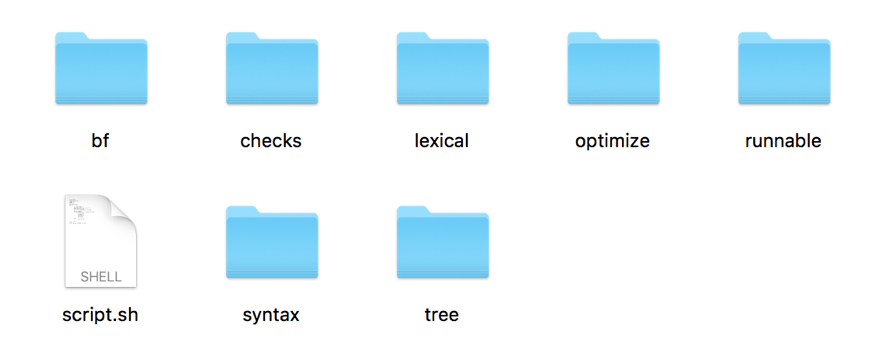
\includegraphics[]{TD/img/folders.png}
	\caption{Suítes de Teste do projeto}
	\label{folders}
\end{figure}

A features da linguagem eram implementadas de acordo com uma estimada ordem de dificuldade.
	
Boa parte do processo de desenvolvimento e do desafio do projeto foi a implementação dos algoritmos disponíveis na Brainfuck Algorithms e o fluxo de trabalho deste mesmo processo.
	
Abaixo há um exemplo de como o fluxo de trabalho de tradução dos algoritmos foi melhorando com o avanço do projeto.

Exemplo:

\begin{verbatim}
    /*   temp0[-]
            y[x+temp0+y-]
            temp0[y+temp0-]*/
\end{verbatim}

Esse é um algoritmo para adição dos valores de duas células (representadas por x e y). Ele é usado no hac para implementar adição entre duas variáveis de 1 byte (isto é, de uma célula). Os nomes presentes nesse algoritmo são, na verdade, abreviações de instruções para ir na célula nomeada de tal forma. (isto é, são abreviações de várias instruções > e <). Neste relatório, tal operação será chamada de goto. (Não confundir com a operação de fluxo de controle. O nome aqui é usado para uma operação referente a acesso a memória). 

É oportuno notar que todo uso da operação goto pode ser resolvido de forma estática. Como a operação goto é recorrente em todos os algoritmos públicos, foi criada uma função para ela:

\begin{verbatim}
    static void codeGoTo(int cellIndex){
        int units = unitsToMoveTo(cellIndex);
        char direction = '>';
        int count = 0;
        assert(currentCell + units == cellIndex)
        if(units < 0){
            direction = '<';
            units = -units;
        }
        currentCell += units;
        
        for( ; units > 0 ; units++){
            count++;
            fprintf(output, "%c" , direction);
        }
        currentCell = cellIndex;
    }
\end{verbatim}

Os algoritmos podem ser implementados por uma composição de impressão de strings com impressões da instrução goto. O algoritmo de adição acima, poderia ser implementado assim:

\begin{verbatim}
    static void incrementXbyY(int x, int y){
        printf("add %d to %d\n" , x, y);
        int temp0 = x - 1;
        codeGoTo(temp0); codeSt("[-]");
        codeGoTo(y); codeSt("["); codeSt(x); codeSt("+");
        codeGoTo(temp0); codeSt("+"); codeSt(y); codeSt("-]");
        codeGoTo(temp0); codeSt("["); codeSt(y); codeSt("+");
        codeGoTo(temp0); codeSt("-]");
    }
\end{verbatim}

Porém, esse estilo de implementação é muito ruim. É muito fácil cometer um erro: é preciso digitar muita coisa para pouco algoritmo. Há também uma grande dificuldade ler e verificar se há um goto para o endereço errado. Isso é particularmente notável quando os algoritmos ficam maiores:

\begin{verbatim}
    static void bfalgo(char* str, ...({
    \\based on http://www.gnu.org/software/libc/manual/html_node/Variadic-Example.html
        va_list ap;
        int i, j, sum;
        
        int count = 0;
        
        for(i = 0 ; str[i] ; i++){
            if(str[i] == '$' || str[i] == '@'){
                count++;
            }
        }
        printf("count %d\n" , count);
        va_start (ap, count);       /*Initialize the argument list.*/
        
        sum = 0;
        for(i = 0 ; str[i] ; i++){
            if(str[i] == '$'){
                int d = va_arg (ap, int);
                codeGoTo(d);
            } else if(str[i] == '@'){ //Not sure if I will use
                char* str = va_arg(ap, char*);
                codeStr(str);
            }
            else {
                fprintf(output, "%c" , str[i]);
            }
        }
        va_end (ap);                /* Clean up. */
    }
    
\end{verbatim}

\begin{verbatim}
    /*
    temp0[-]
    temp1[-]
    temp2[-]
    temp3[-]
    x[temp0+x-]
    temp0[
        y[temp1+temp2+y-]
        temp2[y+temp2-]
        temp1[
            temp2+
            temp0-[temp2[-]temp3+temp0-]
            temp3[temp0+temp1-]
            temp2[
                temp1-
                [x-temp1[-]]+
            temp2-]
        temp1-]
        x+
    temp0]
    */
\end{verbatim}

A solução para esse problema foi a implementação de uma função similar a printf para compor os algoritmos. Esta função recebe um número estaticamente variável de parâmetros (implementados com elipses em C). A função recebe a estrutura do algoritmo, em uma string, e, em seguida, os endereços das variáveis utilizadas para compor o algoritmo.

\begin{verbatim}
    /*   temp0[-]
            y[x+temp0+y-]
            temp0[y+temp0-]*/
            
    static void incrementXbyY(int x, int y){
        int temp0 = x-1;
        bfalgo("$[-] $[$+$+$-] $[$+$-]", temp0, y, x, temp0, y, temp0, y, temp0);
    }
\end{verbatim}

Pode-se observar que ela basicamente mantém o tamanho do texto original do algoritmo e é muito mais simples de ler e verificar se as variáveis estão nos locais corretos.

Embora a função bfalgo() facilitasse bastante o trabalho em relação ao método anterior, os temporários ainda tinham que ser colocados manualmente na chamada, e isso continuava sujeito aos erros do trabalho manual. Além disso a página Brainfuck Algorithms foi atualizada durante o desenvolvimento da Headache e era bastante trabalhoso adicionar manualmente novos algoritmos.

Para solucionar esse problema no fluxo de trabalho foi criado um utilitário chamado bfalgoConverter, que converte os algoritmos no formato da página Brainfuck Algorithms para chamadas da função bfalgo(). 

\begin{figure}[h]
	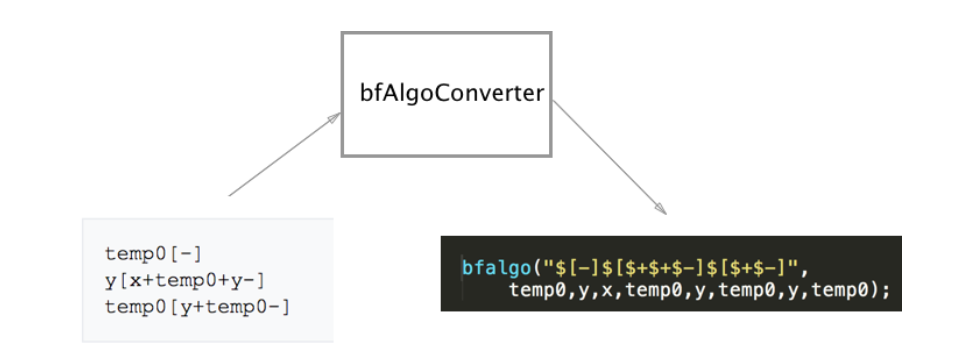
\includegraphics[]{TD/img/bfalgo.png}
	\caption{Esquema do bfalgoConveter}
	\label{folders}
\end{figure}

Ele foi implementado de uma maneira bastante hardcoded, porém, atende o seu propósito:

\begin{verbatim}
    char bigStr[1024*1024];     //1MB
    int tempList[999];
    int * tempListPtr = tempList;
    char* bigStrPtr = bigStr;
    while(fscanf(stdin, "%c" , &c) != EOF){
        if(!isBfChar(c)) {
            if(c == 't') {
                if(fscanf(stdin, "%c" , &c) != EOF){
                    if(c == 'e') {
                        if(fscanf(stdin, "%c" , &c) != EOF){
                            if(c == 'm') {
                                if(fscanf(stdin, "%c" , &c) != EOF){
                                    if(c == 'p'){
                                        if(fscanf(stdin, "%d" , &n) != EOF){
                                            *bigStrPtr = '$';
                                            bigStrPtr++;
                                            *tempListPtr = n;
                                            tempListPtr++;
                                            continue;
                                        }
                                    }
                                }
                            }
                        }
                    }
                }
            }
        }
        else{
            *bigStrPtr = c;
            if(c == 'x');
            ...
        }
    }
    
\end{verbatim} 

\section{Resultado}

Ao final temos, como produtos diretos deste estudo: o repositório de Headache no github; o compilador hac; o interpretador brainfuck bfi; o utilitário expansor de bitwidth expander; o utilitário de conversão dos algoritmos da Brainfuck Algorithms  bfalgoConverter, que converte códigos da webpage para as chamadas da função bfalgo(); a wiki da Headache no github e a EBNF de Headache no Anexo B.

\section{Cronograma}

O desenvolvimento de Headache foi bastante conturbado. Os cronogramas apresentados durante a proposta e durante o projeto final 1 divergem bastante de como foi efetivamente feito.  O desenvolvimento de Headache é público, devido a sua natureza open source, e pode ser verificado e acompanhado na página https://github.com/LucasMW/Headache/commits/master e https://github.com/LucasMW/Headache/graphs/contributors.

As principais diferenças entre os cronogramas se dá na ordem das tarefas e na concentração das tarefas em cada mês. Por exemplo:

A EBNF foi re-elaborada várias vezes; Prints dinâmicos de 8 bits foram concluídos antes de funções (embora prints de 8+ bits acabaram sendo concluídos, de fato, depois); A sintaxe e a AST foram atualizadas próximas ao fim do cronograma; etc.

Cronograma original:

\textbf{2017.1}

Abril:
\begin{itemize}
    \item Coletar /analisar bibliografia
    \item Elaboração da EBNF de Headache
\end{itemize}

Maio:
\begin{itemize}
    \item Descrição do modelo de memória de Headache 
    \item Início dos esboços de implementação
\end{itemize}

Junho:
\begin{itemize}
    \item Elaboração do relatório.
    \item Implementação do Analisador léxico
    \item Implementação do Analisador Sintático
    \item Implementação da Árvore Sintática Abstrata
\end{itemize}

\textbf{2017.2}

Julho:
\begin{itemize}
    \item Implementação de variáveis locais
    \item Completa implementação de expressões	
\end{itemize}

Agosto:
\begin{itemize}
    \item Revisão dos relatórios
    \item Implementação de variáveis globais
    \item Implementação completa da checagem de tipagem	
\end{itemize}

Setembro:
\begin{itemize}
    \item Implementação de funções e calls
    \item Implementação de Condições
    \item Implementação de if / else e while
\end{itemize}

Outubro:
\begin{itemize}
    \item Implementação do print dinâmico 
\end{itemize}

Novembro:
\begin{itemize}
    \item Revisão do código	
\end{itemize}

Extras:
\begin{itemize}
    \item Adicionar arrays tipados 
    \item Otimizar código gerado
\end{itemize}
%%
%
% ARQUIVO: cap-02.tex
%
% VERSÃO: 1.0
% DATA: Maio de 2017
% AUTOR: Carla Cosenza, Matheus Mello, Rebeca Reis
% 
%  Arquivo tex de exemplo de capítulo do documento de Projeto de Fim de Curso.
%
% ---
% DETALHES
%  a. todo capítulo deve começar com \chapter{•}
%  b. usar comando \noindent logo após \chapter{•}
%  c. citações para referências podem ser
%       i. \citet{•} para citações diretas (p. ex. 'Segundo Autor (2015)...'
%       ii. \citep{•} para citações indiretas (p. ex. '... (AUTOR, 2015)...'
%  d. notas de rodapé devem usar dois comandos
%       i. \footnotemark para indicar a marca da nota no texto
%       ii. \footnotetext{•}, na sequência, para indicar o texto da nota de rodapé
%  e. figuras devem seguir o exemplo
%       i. devem ficar no diretório /img e devem ser no formato EPS
%  f. tabelas devem seguir o exemplo
%  g. figuras e tabelas podem ser colocadas em orientação landscape
%       i. figuras: usar \begin{sidewaysfigure} ... \end{sidewaysfigure}
%                   em vez de \begin{figure} ... \end{figure}
%       ii. tabelas: usar \begin{sidewaystable} ... \end{sidewaystable}
%                    em vez de \begin{table} ... \end{table}
%  h. toda figura e tabela deve ser referenciada ao longo do texto com \ref{•}
% ---
%%

\chapter{Projeto e especificação do sistema}
\noindent

Além de seus respectivos fontes, 3 artefatos binários foram criados: hac, bfi e expander. 

\section{hac}

hac é o compilador de Headache para brainfuck. 

\begin{figure}[h]
    \centering
	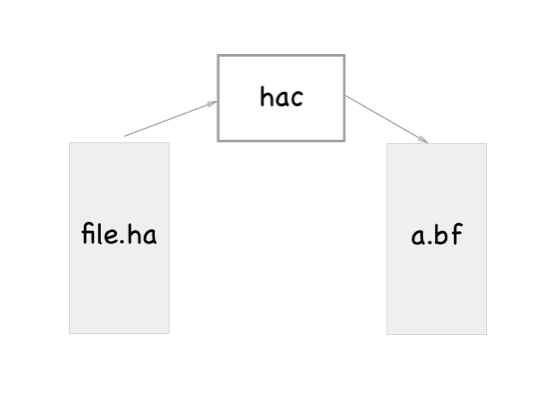
\includegraphics[]{TD/img/hac.png}
	\caption{Esquema simples sobre o hac}
	\label{hac}
\end{figure}

A utilização usual do hac é descrita como:

\begin{verbatim}
    ./hac [opção] file.ha
\end{verbatim}

file.ha é o arquivo source em Headache (.ha) a ser convertido em brainfuck. 

O resultado é sempre salvo em um arquivo nomeado a.bf.

Antes do arquivo source.ha, poderá vir uma opção de interrupção do fluxo de controle.

São elas: 

\begin{itemize}
    \item -lex: roda apenas o analisador léxico.
    \item -syntax: diz se o programa fornecido no input pertence à gramática de Headache.
    \item -tree: Exibe a AST gerada a partir do programa fornecido.
    \item -check: Checa erros e alertas sem compilar o programa.
    \item -noBin: Não executa o interpretador interno após a compilação.
\end{itemize}

Se nenhum programa for fornecido ao hac, ele entrará no "modo interativo", isto é, esperará o programa pela entrada padrão.

Além disso, o hac poderá receber o parâmetro de otimização -O0 ou -O1. Este parâmetro pode vir antes ou depois dos outros parâmetros. Se o parâmetro for -O0, o hac não efetuará nenhuma otimização na AST. Caso -O1 seja fornecido, o hac aplicará otimizações de constantes em tempo de compilação. Isso é feito simplificando operações de constantes na AST. 

Por exemplo: com -O1 expressões como "@1+1+1;" são transformadas em "@3;" na própria AST. 

-O2 transforma operações como "a = a + 3;" em "a+=3", que em brainfuck é apenas "goto(a); +++". Incremento e decremento são nativos em brainfuck, e muito mais rápidos que operações de adição e atribuição, resultando em uma otimização genuína. Essa feature não está corretamente implementada, contudo.

Além disso, o hac também tem as opções --help e --version para a conveniência do usuário.

O hac foi projetado de forma similar ao mongaComp (projeto da disciplina de compiladores). Os códigos estão modularizados de acordo com o seguinte fluxo de execução:

\begin{figure}[h]
    \centering
	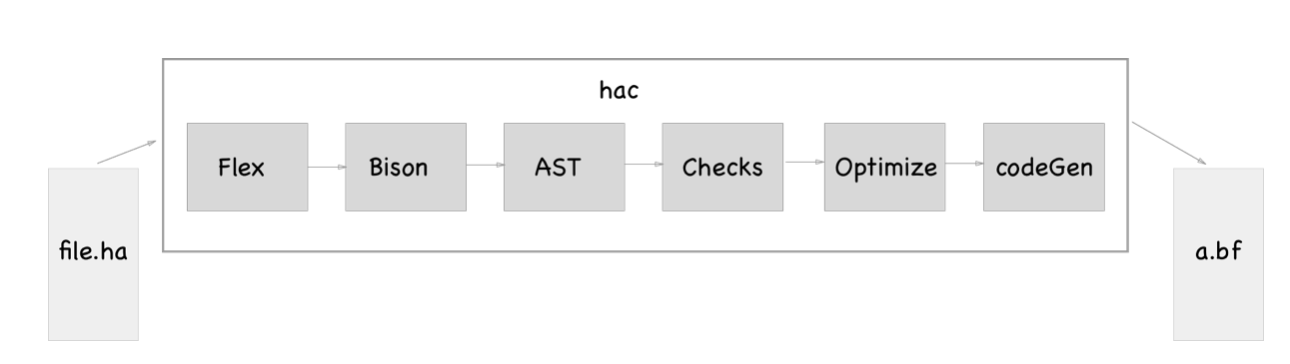
\includegraphics[width = 15cm]{TD/img/esquematicoHac.png}
	\caption{Esquema de funcionamento do hac}
	\label{esquematicoHac}
\end{figure}

O código de input é transformado em tokens; os tokens são avaliados pela gramática, gerando a AST. A AST é checada, tipada. É otimizada, se a opção estiver habilitada e depois é gerado o código output.

bfi (Brainfuck Interpreter) é a versão standalone interpretador de brainfuck utilizado para testes. Uma regra no makefile permite ativar \#ifdef que compila o arquivo testbfi.c com uma main, gerando o bfi. 

\begin{figure}[h]
    \centering
	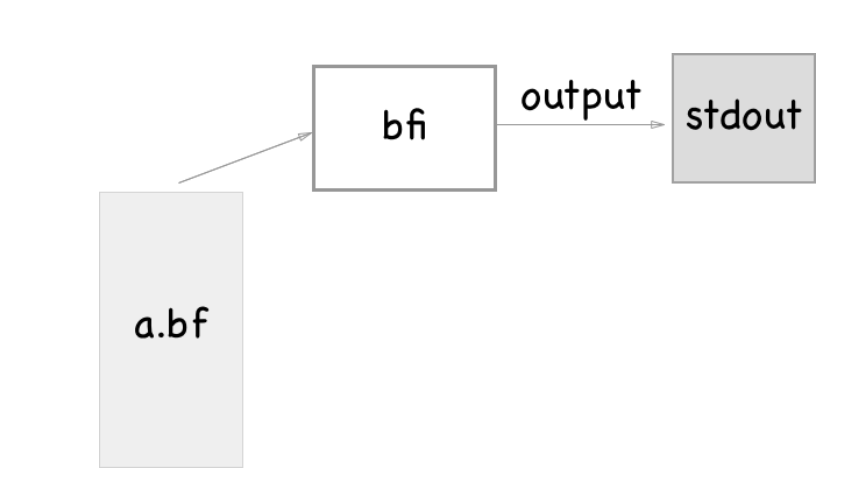
\includegraphics[width = 10cm]{TD/img/bfi.png}
	\caption{Esquema simples sobre bfi}
	\label{bfi}
\end{figure}

\section{bfi}

o bfi é usado da seguinte forma:

\begin{verbatim}
    ./bfi arquivo.bf [-extra]
\end{verbatim}

Isso executa o arquivo brainfuck e imprime na saída padrão. Se o arquivo brainfuck tiver os whiles desemparelhados (instruções '[' e ']'), ele não executa o programa, porém exibe uma mensagem de erro. 

Se a opção -extra for fornecida, o bfi interpreta cada ocorrência do caractere '@' como instrução de debug. Ao encontrar o '@', o bfi exibe o estado atual da memória do interpretador naquele momento da execução. 

A opção "-extra" do bfi faz parte das ferramentas de debug de Headache e está relacionada com a instrução de debug do hac. O comando "\%;"  faz com que o hac gere '@' para que se ative o print da memória naquele momento da execução.

Essas instruções não fazem parte do padrão de brainfuck e portanto só são acionados se os respectivos parâmetros forem fornecidos.

\section{expander}

O expander é um programa para executar extensão de bitwidth de programas brainfuck. Por extensão de bitwidth este documento se refere a transformar um programa em brainfuck de 8 bits em um programa com 16 bits, 32 bits quando executado num interpretador de brainfuck de 8 bits. Isso é obtido por transformar cada instrução em uma sequência maior de instruções. 

\begin{figure}[h]
    \centering
	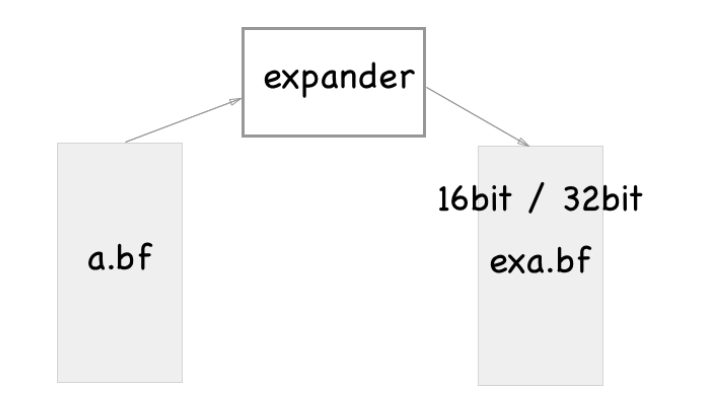
\includegraphics[width = 7cm]{TD/img/expander.png}
	\caption{Esquema simples sobre o expander}
	\label{expander}
\end{figure}

É assim que Headache implementa inteiros de mais de 8 bits. (shorts e ints) .

O expander é utilizado da seguinte forma:

./expander sourcepath [mode]: recebe o path do arquivo brainfuck como input 

ou

./expander -p "source" [mode] : recebe o input entre aspas

ou

./expander -i [mode] : ativa o modo interativo (recebe o input na entrada padrão)

O expander sempre imprime o resultado na saída padrão. 

O parâmetro opcional mode é um inteiro pertencente a {0,1,2}. Cada número representa uma transformada a ser aplicada nas instruções. Os modos 0 e 1 são estratégias diferentes para expandir x2 bits e o modo 2 é para expandir x4 bits.

Um exemplo para entender o funcionamento do expander é:

\begin{verbatim}
    expanding.ha
    void main(){
        byta a;
        a = 200;
        a = a + a;
        @a;@"\n";
    }
    ./hac expanding.ha 
    ./bfi a.bf
    144
\end{verbatim}

Porém se aplicarmos:

\begin{verbatim}
    ./expander a.bf > exa.bf
    ./bfi exa.bf
    400
\end{verbatim}

Ou seja, programa assume o comportamento de:

\begin{verbatim}
    void main(){
        short a;
        a = 200;
        a = a + a;
        @a;@"\n";
    }
\end{verbatim}

Infelizmente, ainda não é possível ao hac expandir apenas as instruções que lidem com shorts, porém, o hac consegue sim compilar programas que tenham shorts: Ao detectar um tipo com mais de 8 bits, uma variável é modificada para saber a quantidade de expansão necessária na main.c; O programa é compilado como se tudo fossem bytes, e  ao final da compilação, o output é expandido.

Os arquivos fontes do expander possuem a macro standalone assim como o bfi. Eles são compilados junto ao hac para que as funções do expander sejam automaticamente chamadas se o hac detectar shorts ou ints no seu input. Isso o torna capaz de gerar output em brainfuck de 8 bits capaz de 16 ou 32 bits.

Contudo, com o uso do expander como programa standalone é perfeitamente possível que um programa feito somente com shorts seja obtido expandido de um programa feito somente com bytes. Inclusive programas brainfuck não gerados pelo hac.

Nenhuma das soluções citadas anteriormente lida com inteiros acima de 8 bits. Até o conhecimento do autor desse projeto, isso é uma exclusividade de Headache.

\section{bfalgoConverter}

Há ainda o bfalgoConverter, mencionado anteriormente. Ele permite traduzir os algoritmos publicados na Brainfuck Algorithms diretamente para chamadas da função bfalgo() (que Headache usa para codificar os algoritmos na hora de gerar o código output).

Como a Brainfuck Algorithms continua a ser atualizada, o bfalgoConverter ajudará futuros colaboradores a adicionar novas features e melhorar as existentes.

\begin{figure}[h]
    \centering
	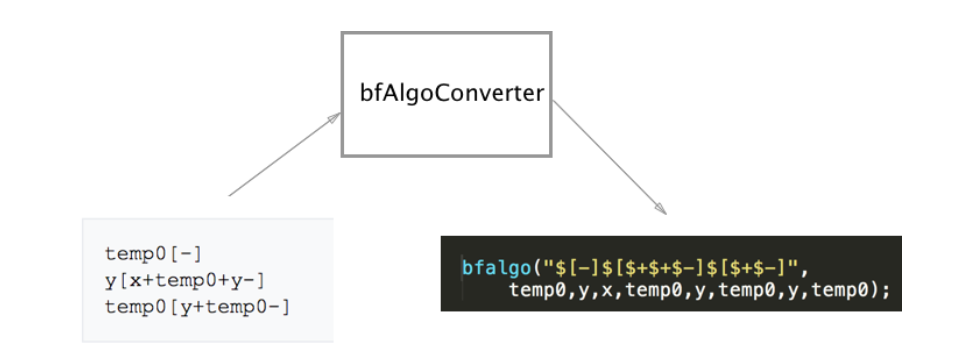
\includegraphics[]{TD/img/bfalgo.png}
	\caption{Esquema do bfalgoConverter}
	\label{Bfalgo}
\end{figure}
%%
%
% ARQUIVO: cap-02.tex
%
% VERSÃO: 1.0
% DATA: Maio de 2017
% AUTOR: Carla Cosenza, Matheus Mello, Rebeca Reis
% 
%  Arquivo tex de exemplo de capítulo do documento de Projeto de Fim de Curso.
%
% ---
% DETALHES
%  a. todo capítulo deve começar com \chapter{•}
%  b. usar comando \noindent logo após \chapter{•}
%  c. citações para referências podem ser
%       i. \citet{•} para citações diretas (p. ex. 'Segundo Autor (2015)...'
%       ii. \citep{•} para citações indiretas (p. ex. '... (AUTOR, 2015)...'
%  d. notas de rodapé devem usar dois comandos
%       i. \footnotemark para indicar a marca da nota no texto
%       ii. \footnotetext{•}, na sequência, para indicar o texto da nota de rodapé
%  e. figuras devem seguir o exemplo
%       i. devem ficar no diretório /img e devem ser no formato EPS
%  f. tabelas devem seguir o exemplo
%  g. figuras e tabelas podem ser colocadas em orientação landscape
%       i. figuras: usar \begin{sidewaysfigure} ... \end{sidewaysfigure}
%                   em vez de \begin{figure} ... \end{figure}
%       ii. tabelas: usar \begin{sidewaystable} ... \end{sidewaystable}
%                    em vez de \begin{table} ... \end{table}
%  h. toda figura e tabela deve ser referenciada ao longo do texto com \ref{•}
% ---
%%

\chapter{Implementação e avaliação}
\noindent

\section{Processo de teste das features implementadas}

As partes referidas ao analisador léxico e sintático são relativamente fáceis de testar. Na main do projeto existem flags para acionar apenas partes específicas do compilador (tal como o gcc e o clang tem essas opções, por exemplo).

Cada suíte de teste tem uma pasta para si. A pasta leva o nome da suíte de teste. Cada suíte de teste é composta por n casos de teste (compostos de um teste.ha e  um teste.answer, onde o .ha representa o input para o compilador e o .answer o resultado produzido esperado) e um script shell script.sh. 

O script é responsável por acionar o compilador com os parâmetros corretos; testar cada um dos casos; comparar a resposta produzida com a resposta esperada e contabilizar o número de testes bem-sucedidos e mal-sucedidos. A diferença entre as respostas é calculada pelo comando diff do Unix e permite verificar exatamente quais são as linhas em que a diferença ocorre.

Ter um script.sh para cada suíte de teste é uma abstração que permite casos de teste mais elaborados: desde testar se o compilador reage a um input incorreto com a mensagem de erro apropriada a compilar e executar inputs fornecidos verificando se a execução está nos conformes.

Finalmente, cada suíte de teste tem uma regra no makefile para facilitar o seu uso. O padrão de nome é test<nome da suíte de teste>. Para executar a suíte de teste lexical, basta digitarmos make testlexical.

Há ainda, uma regra no makefile nomeada test. Ela possui como dependências todas as regras de teste. Com ela, é possível executar todos os testes do projeto simplesmente digitando 'make test' pela linha de comando no diretório raiz do projeto (veja figura \ref{erro}).

\begin{figure}[h]
    \centering
	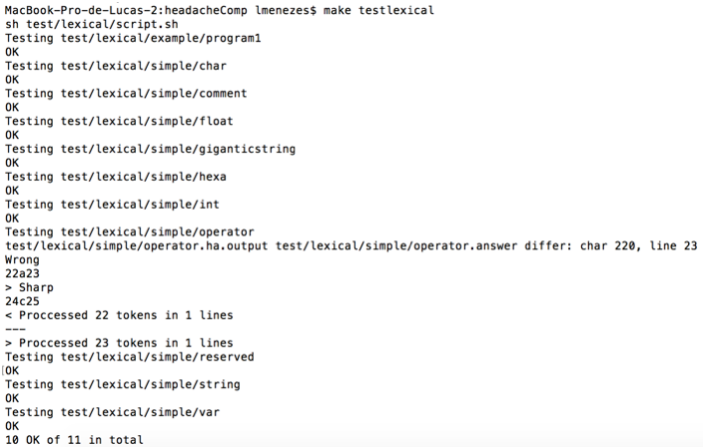
\includegraphics[]{TD/img/erro.png}
	\caption{Exemplo de erro em um arquivo de teste}
	\label{erro}
\end{figure}

\section{Método de debug ou modo run}

Há ainda o método utilizado para depurar a geração de código propriamente dita. Nos arquivos fonte, há um interpretador brainfuck (bfi) utilizado para auxiliar o desenvolvimento. 

Ele é habilitado na main por uma flag, tal como outras opções do compilador. É executado após a compilação e permite ao hac verificar o estado da memória do interpretador após (e, possivelmente, durante) a execução do programa. Isso é especialmente útil para depurar a implementação de variáveis, parâmetros e operações nos seus estados iniciais de desenvolvimento.

Esse modo conta com uma função que busca valores preenchidos na memória do interpretador. Ela é usada para decidir a partir de qual célula o conteúdo da memória será mostrado. 

Apesar desse modo ter sido implementado apenas para fins de debug, ele pode se tornar uma feature do compilador hac. Muitas linguagens de programação permitem, no seu compilador, um modo compile e um modo run.

\begin{verbatim}
    if(!noDebug)
    {
        printf("Debugging\n");
        char* program = readFile(bf_name);
        printf("exec\n");
        int used = execute(program, 30000, 1);
        free(program);
        printf("printing memory\n");
        printAllWrittenMemory();
        printf("used %d cells (bytes) to run\n", used);
    }
    
    Debugging
    exec
    144
    11
    222
    1
    printing memory
    start 0: |0|0|0|0|0|0|144|11|222|1|0|0|0|2|11|0|30|33|
    start 18: |0|64|0|0|1|0|0|0|0|0|0|0|0|0|0|0|
    used 36 cells (bytes) to run
\end{verbatim}

Apesar desse modo ter sido implementado apenas para fins de debug, ele pode se tornar uma feature do compilador hac. Muitas linguagens de programação permitem, no seu compilador, um modo compile e um modo run.

Alguns exemplos de programas que o hac pode transformar em brainfuck:

\begin{verbatim}
------ example.ha -------
void main() {
	@"Hello World!\n";
}
----- sub.ha -----
void main() {
	byte a;
	byte b;
	byte c;
	a = 3-1+7; 
	b = a-10;
	c = 21;
	c = c - 256;
-------divide.ha -------
void main(){
	byte a;
	byte b;
	byte c;
	byte d;
	a = (10*6+3)/7; /* 63/7 = 9 */
	b = (10*23-5*23)/23; /* 5*23/23 = 5 */
	c = 0/0+10/10; /* 0/0 converts to zero in headache */
	d = a/a + b/b + c/c;
	@"a: "; @a; @"\n";
	@"b: "; @b; @"\n";
	@"c: "; @c; @"\n";
	@"d: "; @d; @"\n";
}


-------conditions.ha ------- 
void main() {
	byte a;
	a = 10;
	if(a>1) { 
		if(a>2){ 
			if(a>3) { 
				if(a>4){ 
					if(a>5){ 
						@a;@" is greater than five\n";
					}
					@a;@" is greater than four\n";
				}
				@a;@" is greater than three\n";
			}
			@a;@" is greater than two\n";
		} 
		@a;@" is greater than one\n";

	} else if(true) {
		@"Block 1";@"\n";
	} else if(2==2) {
		@"Block 2";@"\n";
	} else if(3<4) {
		@"Block 3";@"\n";
	}
}

-------count.ha -------
void main()
{
	byte a;
	a=1;
	while(a){
		@a;@"\n";
		a++;
	}
}
-------while2.ha -------
void main(){
	byte i,j;
	byte x,y,r;
	i = 2;
	r = 0;
	while(i){
		j=2;
		while(j){
			//@"y ";
			j--;
			r++;
		}
		i--;
		//@"x\n";
	}
	@"Result is "; @r; @"\n";
}




-------power.ha -------
short pow(short x, short y){
	short r,z;
	r=1;
	z = y;
	while(z){
		r = r*x;
		z--;
	}
	return r;
}
void main(){
	short a,b;
	a=2;
	b=10;
	@"pow(";@a;@",";@b;@") = ";
	@pow(a,b);@"\n";
}

\end{verbatim}

\section{Comentários sobre implementação}

Para fazer com que a main() executasse, ela é a única função cuja definição é compilada (forçando um call).

FIGURA/CODIGO

A existência desse tipo de exceção me leva a crer que não existe nenhuma boa razão para não incluir um modo interativo em Headache tal qual linguagens como Lua e Python. É muito provável que a estrutura do código ficasse até mais fluída.

\section{Comentários sobre defeitos}

Dentre os problemas encontrados temos:

\begin{itemize}
    \item Organização de código no codegen.c: Módulo muito grande que além de conter código desnecessário é pouco modularizado. Sugestão: Separar as funções que implementam os algoritmos da Brainfuck Algorithms da transformação da AST em código output. Status: Não implementado.
    \item Corrupção de registradores por condições em loops while. Solução proposta: adicionar registradores ou compilar todas as variáveis e temporários para endereços estáticos em tempo de compilação. Status: Não implementado completamente. Há bugs.
    \item Combinar a geração de código para tipos byte e short de forma nativa não foi feito. Ao invés, foi adotada uma solução alternativa: detectar se o programa usa shorts e ativar uma flag; Compilá-lo usando apenas variáveis bytes e expandir o programa todo ao final. Isso gera uma semântica diferente (algumas variáveis em short contra todas em short), porém permite, em versão beta, a feature de shorts em brainfuck
\end{itemize}

\section{Features pensadas porém não implementadas}

\begin{itemize}
    \item tipo bit
\end{itemize}

Ter um tipo próprio para operações booleanas, um tipo que só pudesse assumir os valores 0 e 1 e que essa propriedade fosse checada estaticamente (em tempo de compilação). Se não faz diferença nos registradores usuais das CPUs essa diferença, em brainfuck certamente faz (menos incrementos e decrementos, algoritmos de checagem mais rápidos). Esse tipo seria conveniente denominado bit (para fazer par ao tipo byte)

\begin{itemize}
    \item tipo float/real
\end{itemize}

Implementar o tipo real/float baseando-se na implementação antiga do tipo real em pascal, (quando ainda não era implementado em hardware, mas utilizando libs de algortimos de manipulação de bits). Foi cortado do projeto devido a estar claramente fora do escopo do tempo.

\begin{itemize}
    \item inline brainfuck
\end{itemize}

Permitir que o programador, ao escrever código Headache, tivesse alguma estrutura que o permitisse otimizar um processamento com o seu próprio código brainfuck.

\begin{itemize}
    \item ibs e include
\end{itemize}

Permitir a inclusão de libs com funções comuns como print(), println(), pow(x,y), sqrt(x). 

O programador Headache escreveria no topo do documento algo como "include stdprint" para utilizar a println(). Escreveria algo como “include stdmath” para utilizar a pow() e a sqrt(). Poderia incluir o tipo real/float  com algo como include “stdreal”.

Headache podia ter um diretório Headers/ com o código em Headache dessas libs (stdprint.ha, stdmath.ha), que seria, por baixo dos panos, colado no topo do documento e compilaria normalmente.

\begin{itemize}
    \item for
\end{itemize}

for ao estilo C como açúcar sintático para o while foi planejado. Porém devido a dificuldades de implementação, ele é representado de uma forma diferente na AST e sua geração de código é independente. \newline


Como se pode observar, muitas dessas features que não chegaram a ser incluídas seriam utilizadas juntas, ou uma ajudaria a implementar a outra.

%%
%
% ARQUIVO: cap-02.tex
%
% VERSÃO: 1.0
% DATA: Maio de 2017
% AUTOR: Carla Cosenza, Matheus Mello, Rebeca Reis
% 
%  Arquivo tex de exemplo de capítulo do documento de Projeto de Fim de Curso.
%
% ---
% DETALHES
%  a. todo capítulo deve começar com \chapter{•}
%  b. usar comando \noindent logo após \chapter{•}
%  c. citações para referências podem ser
%       i. \citet{•} para citações diretas (p. ex. 'Segundo Autor (2015)...'
%       ii. \citep{•} para citações indiretas (p. ex. '... (AUTOR, 2015)...'
%  d. notas de rodapé devem usar dois comandos
%       i. \footnotemark para indicar a marca da nota no texto
%       ii. \footnotetext{•}, na sequência, para indicar o texto da nota de rodapé
%  e. figuras devem seguir o exemplo
%       i. devem ficar no diretório /img e devem ser no formato EPS
%  f. tabelas devem seguir o exemplo
%  g. figuras e tabelas podem ser colocadas em orientação landscape
%       i. figuras: usar \begin{sidewaysfigure} ... \end{sidewaysfigure}
%                   em vez de \begin{figure} ... \end{figure}
%       ii. tabelas: usar \begin{sidewaystable} ... \end{sidewaystable}
%                    em vez de \begin{table} ... \end{table}
%  h. toda figura e tabela deve ser referenciada ao longo do texto com \ref{•}
% ---
%%

\chapter{Considerações finais}
\noindent

\section{Contribuições desse trabalho para a comunidade}
Usuários e criadores linguagens esotéricas se animaram com o trabalho. O repositório de Headache teve um fork do criador da brain-lang (uma extensão de brainfuck com mais comandos, não confundir com o projeto homônimo similar à Headache)  para adaptar o hac para que este compilasse para brain. Headache também teve uma entrada (escrita por mim) na esolangs.org. 

Conforme foi mencionado anteriormente, a "pesquisa em brainfuck” continua ocorrendo: A Brainfuck Algorithms recebe novos códigos; otimizadores de brainfuck são criados; projetos similares a Headache surgiram no mesmo ano, mesmo sem contato comum conhecido; e outras linguagem esotéricas baseadas em brainfuck continuam a ser criadas.

Headache coroa como uma dessas pesquisas, com atualmente 14 estrelas no github. (Sexto lugar na pesquisa “esoteric-programming-language” ; Décimo-quinto na pesquisa “esolang” e décimo terceiro na tag “brainfuck” - quando o relatório foi escrito).

Se Headache alcançar 50 estrelas no github, pode ser considerado famoso o suficiente para figurar no Homebrew: o package manager não oficial do mac OS (segundo o critério do Homebrew para criar novos pacotes) .

\section{O que foi aprendido}
Melhor domínio do git. Manusear forks públicos no github. Extensão de bitwidth em brainfuck. Uso de elipses em C. Otimização básica de constantes. Redigir make install. Redigir interpretação de parâmetro; Redigir testes que envolvessem a execução de de código gerado. Utilizar o minGW para compilar programas C Unix no Windows.

Se eu começasse a fazer Headache hoje, pensaria em implementá-la em rust contra implementá-lo em C. Mas o mais importante é que eu faria o source do zero ao invés de começar a trabalhar a partir do source do mongaComp, apenas utilizando-o para consulta. Por mais que tenha me permitido refatorar o código do projeto original, isso acabou acoplando código desnecessário ao hac que acabou passando às revisões. O código poderia ser muito reduzido se isso não tivesse sido feito. 

Também o faria direto numa implementação sem registradores, baseada apenas no uso de heap fixo e liberado após cada execução, tudo calculado estaticamente (no momento de compilação).


\section{Oportunidades para trabalhos futuros}
Um próximo aluno poderia resolver os bugs do hac ou implementar mais features. Headache abre espaços para receber muitas contribuições de tipos diferentes: 

Implementar novas features na linguagem, por exemplo: 

Arrays dinâmicos; 

Variáveis real; 

(Existe uma lista de features planejadas que não chegaram a ser implementadas neste mesmo relatório). Seriam todas extremamente bem vindas a integrar o repositório.

Implementar novas otimizações em -O1 -O2 ou -O3.

Otimizar o código do hac. 

Nota: Há uma diferença entre otimizar os algoritmos e o modelo de memória que Headache se baseia para gerar o código output e adicionar otimizações de AST (que é o que é ativado nas opções -O1, -O2, -O3). As otimizações de AST são, basicamente, conversões de conjuntos de instruções em conjuntos menores e mais rápidos que tenham o mesmo efeito ainda dentro da representação interna do compilador (Headache -> Headache). É diferente de otimizar a geração de código, isto é, como certas estruturas da linguagem são transformadas em código output.

Fazer um fork no repositório github para que Headache seja compilada em uma variante de brainfuck, ou outra linguagem esotérica como whitespace.

Headache foi concebida para ser open source e receber pull requests de vários colaboradores. Há muitos ramos diferentes que podem ser explorados por uma aluno que queira realizar melhorias

\phantom{\cite{Peres}, \cite{Pegg}, \cite{Clifford}, \cite{Hughes}, \cite{Github}, \cite{Libbf}, \cite{BrainfuckCode}, \cite{BrainfuckUtil}, \cite{GoogleCode}, \cite{BFO}, \cite{BrainfuckDummies}, \cite{BrainfuckA}, \cite{Brainfuck}}


% -----
% PARTE DE REFERÊCIAS BIBLIOGRÁFICAS DE PFC
%
%  As referências do documento de PFC devem estar no arquivo refs.bib
%  Devem seguir o formato bibtex - ver Manual-Referencias.pdf para mais detalhes.
% -----
\bibliographystyle{pfc}
\bibliography{refs}

% -----
% PARTE DE APÊNDICE DE PFC
%
%  Se o documento de PFC não tiver apêndices REMOVER AS LINHAS ABAIXO
%  Adicionar os arquivos .tex de apêndice ao documento com comando \include{•}
% -----

% -----
% PARTE DE ANEXO DE PFC
%
%  Se o documento de PFC não tiver anexos REMOVER AS LINHAS ABAIXO
%  Adicionar os arquivos .tex de anexo ao documento com comando \include{•}
% -----
\inannex
%%
%
% ARQUIVO: anexo.tex
%
% VERSÃO: 1.0
% DATA: Maio de 2016
% AUTOR: Coordenação de Trabalhos Especiais SE/8
% 
%  Arquivo tex de exemplo de anexo do documento de Projeto de Fim de Curso.
%  Este exemplo traz dois anexos (dois comandos \chapter{•}). Poderiam ser colocados em arquivos .tex
%  separados. Neste caso, o arquivo main.tex deveria ter um \include{•} para cada arquivo .tex
%
% ---
% DETALHES
%  a. todo anexo deve começar com \chapter{•}
%  b. usar comando \noindent logo após \chapter{•}
%  c. segue os mesmos DETALHES do arquivo .tex de exemplo de capítulo do documento de Projeto de Fim de Curso
% ---
%%
\chapter{Descrição não formal da linguagem}
\noindent

LINGUAGEM HEADACHE (v 0.51b):\\
Formato livre \\
\textbf{Variáveis:} \\
tipos: byte, short e int. \\
\textbf{Constantes:}\\
tipos: byte e string.\\
\textbf{Funções:} 
\begin{verbatim}
    ret-type fuctionName(type parameter,…)
    void functionName(type parameter,…)
\end{verbatim} \\
\textbf{Operações:}

+,-,*,/,++,--  (byte,byte)

+,-,*,/,++,--  (short,short)

+,-,*,/,++,--  (int,int)

Nota: ++ e -- são comandos e não expressões.

Operações com inteiros que resultem em overflow são continuadas partindo do valor mínimo ou máximo.  \\
\textbf{Print}
\begin{verbatim}
    @ “string" 
    @int    //imprime inteiro 
    @byte   //imprime caractere ascii   
\end{verbatim}\\
autocast para int em caso de short.\\
\textbf{Input}
\begin{verbatim}
    #variável: lê da entrada padrão e adapta os bytes lidos ao tipo da variável 
    #byte //como caractere 
    #string //como string 
    #int //como inteiro 
\end{verbatim}\\
\textbf{Comandos:}
\begin{verbatim}
    if(condição) { 
        //Código 
    } 
    if (condição) { 
        //Código 
    } 
    else { 
        //Código 
    } 
    while(condição) { 
        //Código 
    } 
    for(begin;condição;end){ 
        //Código 
    } 
\end{verbatim}
\textbf{Condições:}
\begin{verbatim}
    int == int 
    int > int 
    int < int 
    int >= int 
    int <= int 
    int != int 
    cond && cond 
    cond || cond 
    (auto cast) 
\end{verbatim}
\textbf{Calls:}
\begin{verbatim}
   functionName(Arguments);  
\end{verbatim}\\
\textbf{Modelo de memória:} 

Funções estáticas inline.  

Não há recursão.

Cada definição de função reserva a área da função. 

A área da função é composta de suas variáveis, mais a área necessária para os temporários de suas expressões.

Parâmetros são transformados em variáveis ordinárias. 

Não há ponteiros. 

Não há memória dinâmica.



\chapter{EBNF de Headache}
\noindent
program: {definition}\\
definition: def-var | def-func\\
def-var : type nameList ';'\\
nameList: ID { ',' ID }\\
type : baseType | type '[' ']'\\
baseType : byte | short | int \\
command:

\begin{verbatim}
    IF '(' exp ')' command [ ELSE command ]
    | WHILE '(' exp ')' command
    | FOR (command; exp; command)
    | var '=' exp ';'
    | RETURN [ exp ] ';'
    | call ';'
    | '@' exp ';'
    | var++;
    | var--;
    | '#' var ‘;’
    | ‘%' ‘;'
    | block

    var : ID | exp '[' exp ']'
    exp : NUMERAL | LITERAL
    | var
    | '(' exp ')'
    | call
    | exp 'as' tipo
    | '-' exp
    | exp '+' exp
    | exp '-' exp
    | exp '*' exp
    | exp '/' exp
    | exp '==' exp
    | exp '<=' exp
    | exp '>=' exp
    | exp '<' exp
    | exp '>' exp
    | '!' exp
    | exp '&&' exp
    | exp '||' exp
    call: ID '(' expList ')'
    expList : [ exp { ',' exp } ]
\end{verbatim}

\chapter{Descrição breve de brainfuck}

Brainfuck é uma linguagem de programação Turing Complete composta por apenas 8 caracteres. São eles: ‘>’, ‘<’ , ‘+’, ‘-’, ‘,’ , ‘.’ , ‘[’, ‘]’ 
Cada um deles representa um comando específico. São eles:

>\hspace*{1.5cm}ir a direita

<\hspace*{1.5cm}ir a esquerda

+\hspace*{1.5cm}incrementar corrente

-\hspace*{1.5cm}decrementar corrente 

,\hspace*{1.5cm}input na célula corrente

.\hspace*{1.5cm}output na célula corrente

[\hspace*{1.5cm}abre while loop

]\hspace*{1.5cm}fecha while loop


Um programa Brainfuck roda numa memória compostas de células de 8 bits. A especificação mais comum é uma memória de 30000 células de 8 bits. Quando um programa começa a memória deve estar com todas as suas células zeradas, e a célula corrente deve ser a célula de número zero. A especificação também prevê que não haja nenhuma célula à esquerda da célula zero: Uma instrução ‘<’ quando o programa está na célula zero de memória deve gerar um erro em um interpretador de brainfuck.
Um programa brainfuck com loops  ('[ ' e ']') desbalanceados são undefined behavior em brainfuck. No artefato bfi implementado, a decisão foi gerar um erro.
Formalmente, brainfuck é definida com a seguinte tradução para C:

\begin{figure}[h]
    \centering
	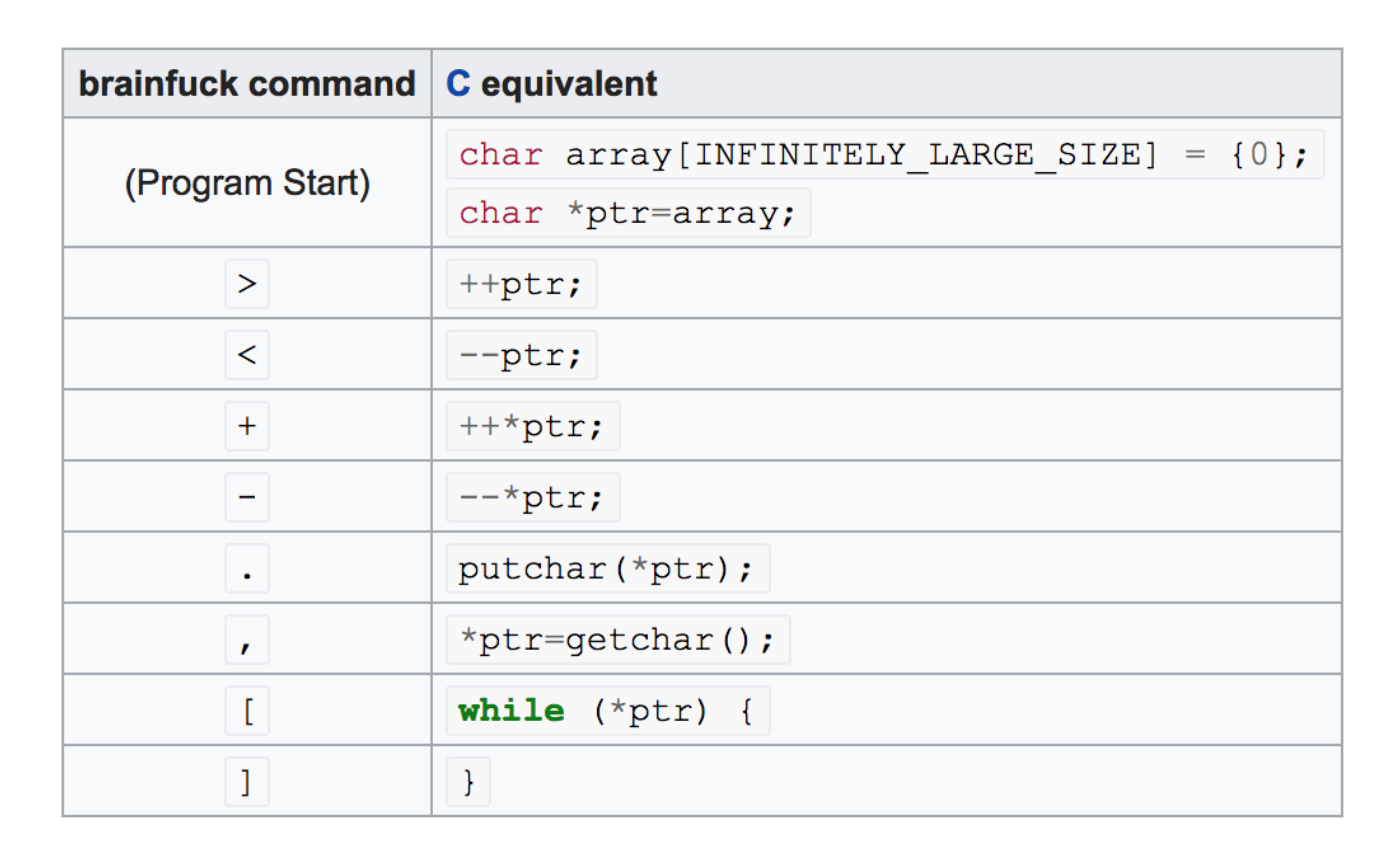
\includegraphics[width = 10cm]{TD/img/C.png}
	\caption{Tradução do brainfuck para o C}
	\label{traducao}
\end{figure}

\chapter{Instruções de Uso}

Essa instrução é dedicada àqueles que executarão o código no CD

\begin{itemize}
    \item Ler o README.txt
    \item Para rodar o "make testrunnable" no linux é necessário executar "git checkout linux" 
    \item Consultar a wiki de Headache em caso de dúvida (https://github.com/LucasMW/Headache/wiki)
    \item Digitar "git pull" para atualizar o projeto
\end{itemize}
\outannex

% -----
% FIM DO DOCUMENTO DE PFC
% -----
\label{theend}
\end{document}
